
\section{Characteristics of Partial Tree}
\label{sec:chars}

Now we discuss the Characteristics of partial trees. Since the left-open nodes,
right-open nodes and pre-nodes are most significant concept in partial trees, we
first focus on the properties of these open node.

\subsection{Properties of Open Nodes}

We introduce three properties of open nodes. The first property is about the
parent-child relationship of the open nodes.

\begin{property}
\label{property1}\itshape
If a node on a partial tree is left/right open, then its parent is also
left/right open.
\end{property}

The second property is about the sibling relationship of the open nodes.

\begin{property}
\label{property2}\itshape
If a node is left open, it is the first node among its
siblings in the partial tree. If a node is right open, it is the last
node among its siblings in the partial tree.
\end{property}

There is another important property of pre-nodes.

\begin{property}
\label{property3}\itshape
If there exist multiple pre-nodes, then only one of
them has left-open/closed/right-open nodes as its child.
\end{property}


\subsection{Standard Structure}

According the properties of partial tree, the standard structure of partial tree
can be described as in Fig.~\ref{fig:model}.

\begin{figure}[t]
\centering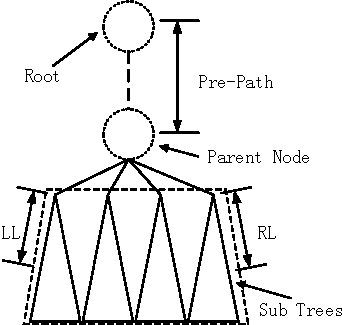
\includegraphics{partialtree/figures/fromWord-4.pdf}
\caption{The standard structure of partial tree.}
\label{fig:model}
\end{figure}

A partial tree consists vertically of two parts. The bottom part is a forest
of subtrees and the top part is a list of pre-open nodes denoting the path from
the root to the bottom part. We call the list of pre-open nodes emph{pre-path}.
Pre-path plays an important role in applying queries from the root. From
property~\ref{property3}, one or more subtrees connect to a pre-node at the
bottom of the pre-path. Note that for each subtree, there is only one root,
which is a left-open/closed/right-open node, but there could be one or more
subtrees.

From properties \ref{property1} and \ref{property2}, we know that left-open
nodes are located on the upper-left part of a partial tree and the right-open
nodes are located on the upper-right part. More precisely, the left-open nodes
form a list from a root node of a subtree, and we call the list the \emph{left
list} (LL). Likewise, we call the list of right-open nodes the \emph{right list}
(RL).
